\documentclass{article}
\usepackage[T1]{fontenc}
\usepackage{lmodern}
\usepackage{amssymb,latexsym,amsmath,stmaryrd,dk,dkenv}
\usepackage{tikz}
\usepgflibrary{shapes}
\usetikzlibrary{arrows,automata,backgrounds}
\usepackage{bbm}

\usepackage[all]{xy}
\usepackage{algorithm}
\usepackage[noend]{algpseudocode}

\DeclareFontFamily{U}{mathb}{\hyphenchar\font45}
\DeclareFontShape{U}{mathb}{m}{n}{<5> <6> <7> <8> <9> <10> gen * mathb <10.95> mathb10 <12> <14.4> <17.28> <20.74> <24.88> mathb12}{}
\DeclareSymbolFont{mathb}{U}{mathb}{m}{n}
\DeclareMathSymbol\fsmash\mathbin{mathb}{"0C}

\newcommand\den[1]{\llbracket #1\rrbracket}
\newcommand\rsem[1]{[#1]}
\newcommand\lsem[1]{L\den{#1}}
\newcommand\cset[1]{\{#1\}}
\newcommand\Rel{\kw{Rel}}
\newcommand\KL{\kw{Kl}}
\newcommand\KLP{\ensuremath{\KL\,\PP}} 
\newcommand\lam[2]{\lambda{#1}\kern1pt.\kern1pt{#2}}
\newcommand\nf[1]{#1^{\mathrm{nf}}}
\newcommand\CA{\ensuremath{P}}
\newcommand\At{\ensuremath{\mathit{At}}}
\newcommand\cseq[2]{\pseq{\pseq{#1}\cdots}{#2}}
\renewcommand\smash{\mathrel{\diamond}}
\newcommand\ssum{\mathop{\textstyle\sum}}
\newcommand\sbigcup{\mathop{\textstyle\bigcup}}
\newcommand\pdup{\mathop{\mathsf{dup}}}
\newcommand\One{\mathbf{1}}
\newcommand\Two{\mathbf{2}}
\newcommand\Exp{\mathsf{Exp}}
\newcommand\bval[1]{[#1]}
\renewcommand\star{^{\textstyle *}}
\newcommand\id{\mathsf{id}}
\newcommand\NetHKC[2]{\texttt{NetKATEquiv}(#1,#2)}
\newcommand\pair[2]{\langle #1,#2\rangle}
\renewcommand\powerset[1]{2^{#1}}
\newcommand\JI{\At\cdot(P\cdot\pdup)\star\cdot P}
\newcommand\setJI{2^{\At\cdot P\cdot(\pdup\cdot P)^{\scriptstyle *}}}
\newcommand\funJI{(2^{\At \cdot P})^{(P\cdot\pdup)^{\scriptstyle *}}}
\newcommand\acc{\mathsf{Accept}}
\newcommand\clname{\mathrm{cl}}
\newcommand\cl[1]{\clname(#1)}

\begin{document}

\begin{namedtheorem}{Theorem 0.2}
$G(e) = G(M_e)$.
\end{namedtheorem}

\begin{definition}
{\it Reduced NetKAT} is a subset of NetKAT where policies are a regular 
expression over atoms, complete assignments, and $\pdup$. Every NetKAT policy 
is provably equivalent to a reduced NetKAT policy.
\end{definition}

\begin{proof} Proof by induction on following the recursive definition of 
reduced NetKAT.

\begin{description}

\item[Idea.] Since all expressions in reduced NetKAT can be seen as a regular 
expression over the alphabet $P \cup A \cup \{\pdup\}$, it will suffice to show
that:
\begin{itemize}
  \item $G(\alpha) = G(M_\alpha)$
  \item $G(\pi) = G(M_\pi)$
  \item $G(\pdup) = G(M_{\pdup})$
  \item For any NetKAT$_{\textnormal{DM}}$ expressions $e_1$ and $e_2$: if
  $G(e_1) = G(M_{e_1})$ and $G(e_2) = G(M_{e_2})$, then 
  $G(e_1+e_2) = G(M_{e_1+e_2})$, $G(e_1;e_2) = G(M_{e_1;e_2})$, and
  $G(e_1\star) = G(M_{e_1\star})$.
\end{itemize}
   
  
\item[Basis Step.]
\mbox{ }
  
\begin{itemize}
  \item $\alpha$:
  \begin{figure}[H]
    \centering
    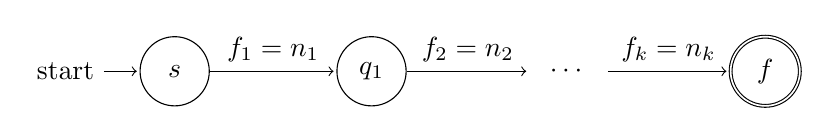
\begin{tikzpicture}[shorten >=1pt, auto]
      %\draw[help lines] (0,-3) grid (10,3);
      \draw (5,0) node {$\cdots$};
      \node[state, initial]   (s)               {$s$};
      \node[state]            (q1) at (2.5,0)   {$q_1$};
      \node[state, accepting] (f)  at (7.5,0) {$f$};
  
      \path[->] (s)  edge node {$f_1=n_1$} (q1)
                (q1) edge node {$f_2=n_2$} (4.5,0)
                (5.5,0) edge node {$f_k=n_k$} (f);
                
    \end{tikzpicture}
    \caption{$M_{\alpha}$}
  \end{figure}
  
  In $M_\alpha$, there is only one path from a start state to an accepting 
  state: $y\equiv f_1=n_1;\cdots;f_k=n_k$. By definition, $G(M_\alpha) = $
  $\{x\ |\ x\leq y$ and $x \in \JI \}$.
  
  \begin{align*}
  y &\equiv f_1=n_1;\cdots;f_k=n_k \\
    &\equiv \alpha & \alpha \triangleq f_1=n_1;\cdots;f_k=n_k \\
    &\equiv \alpha;\pi_{\alpha} & \alpha \equiv \alpha;\pi_\alpha
  \end{align*}

  Since $y \equiv \alpha;\pi_{\alpha} \in \JI$, 
  $x \leq y \implies x \in \{\alpha;\pi_\alpha\}$. Hence, 
  $G(M_\alpha) = \{\alpha;\pi_\alpha\} = G(\alpha)$.

  \item $\pi$:
  \begin{figure}[H]
    \centering
    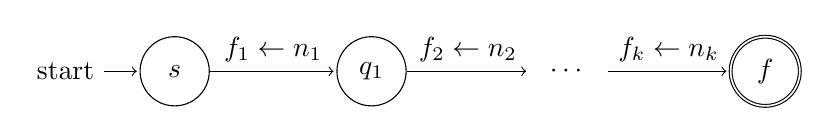
\begin{tikzpicture}[shorten >=1pt, auto]
      %\draw[help lines] (0,-3) grid (10,3);
      \draw (5,0) node {$\cdots$};
      \node[state, initial]   (s)               {$s$};
      \node[state]            (q1) at (2.5,0)   {$q_1$};
      \node[state, accepting] (f)  at (7.5,0) {$f$};
  
      \path[->] (s)  edge node {$f_1 \gets n_1$} (q1)
                (q1) edge node {$f_2 \gets n_2$} (4.5,0)
                (5.5,0) edge node {$f_k \gets n_k$} (f);
                
    \end{tikzpicture}
    \caption{$M_{\pi}$}
  \end{figure}
  
  In $M_\pi$, there is only one path from a start state to an accepting 
  state: $y\equiv f_1 \gets n_1;\cdots;f_k \gets n_k$. By definition, 
  $G(M_\pi) = \{x\ |\ x\leq x \in \JI \}$.
  
  \begin{align*}
  y &\equiv f_1 \gets n_1;\cdots;f_k \gets n_k \\
    &\equiv \pi & \pi \triangleq f_1 \gets n_1;\cdots;f_k \gets n_k \\
    &\equiv \id;\pi & \id;p \equiv p \\
    &\equiv \displaystyle \sum_\alpha \alpha;\pi & \displaystyle \sum_\alpha
      \alpha \equiv \id
  \end{align*}
  
  Since $x \leq p+q \implies x \leq p \vee x \leq q$, 
  $x \leq y \implies \exists \alpha \in At,\ x \leq \alpha;\pi$
  
  , if $x \leq y$, then $x \in \{\alpha;\pi\ |\ \alpha \in At\}$. Hence, 
  $G(M_\pi) = \{\alpha;\pi\ |\ \alpha \in At\} = G(\pi)$.
  
  \item $\pdup$:
  \begin{figure}[H]
    \centering
    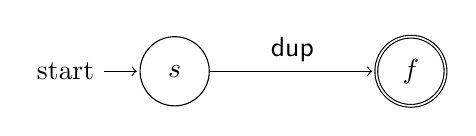
\begin{tikzpicture}[shorten >=1pt, auto]
      \node[state, initial]   (s)           {$s$};
      \node[state, accepting] (f) at (3,0)  {$f$};
  
      \path[->] (s) edge node {$\pdup$} (f);
    \end{tikzpicture}
    \caption{$M_{\pdup}$}
  \end{figure}
  
  In $M_{\pdup}$, there is only one path from a start state to an accepting 
  state: $y\equiv \pdup$. By definition, $G(M_{\pdup}) = $
  $\{x\ |\ x\leq y$ and $x \in \JI \}$.
  
  So, 
  
  \begin{align*}
  y &\equiv \pdup \\
    &\equiv \id;\pdup & \id;p \equiv p \\
    &\equiv \displaystyle \sum_\alpha \alpha;\pdup & \displaystyle \sum_\alpha 
      \alpha \equiv \id \\
    &\equiv \displaystyle \sum_\alpha \alpha;\pi_\alpha;\pdup & \alpha \equiv
      \alpha;\pi_\alpha \\
    &\equiv \displaystyle \sum_\alpha \alpha;\pi_\alpha;\alpha;\pdup & \pi 
      \equiv \pi;\alpha_\pi \\
    &\equiv \displaystyle \sum_\alpha \alpha;\pi_\alpha;\pdup;\alpha & 
      \alpha;\pdup \equiv \pdup;\alpha \\
    &\equiv \displaystyle \sum_\alpha \alpha;\pi_\alpha;\pdup;\alpha;\pi_\alpha
      & \alpha \equiv \alpha;\pi_\alpha \\
    &\equiv \displaystyle \sum_\alpha \alpha;\pi_\alpha;\alpha;\pdup;\pi_\alpha
      & \alpha;\pdup \equiv \pdup;\alpha \\
    &\equiv \displaystyle \sum_\alpha \alpha;\pi_\alpha;\pdup;\pi_\alpha & 
      \pi \equiv \pi;\alpha_\pi
  \end{align*}
\end{itemize}
  
\item[Inductive Step.] For any reduced NetKAT expressions $p$ and $q$: if 
$G(p) = G(M_{p})$ and $G(q) = G(M_{q})$, then $G(p+q) = G(M_{p+q})$, 
$G(p;q) = G(M_{p;q})$, and $G(p\star) = G(M_{p\star})$.

\begin{itemize}
  \item $p+q$:
  \begin{figure}[H]
    \centering
    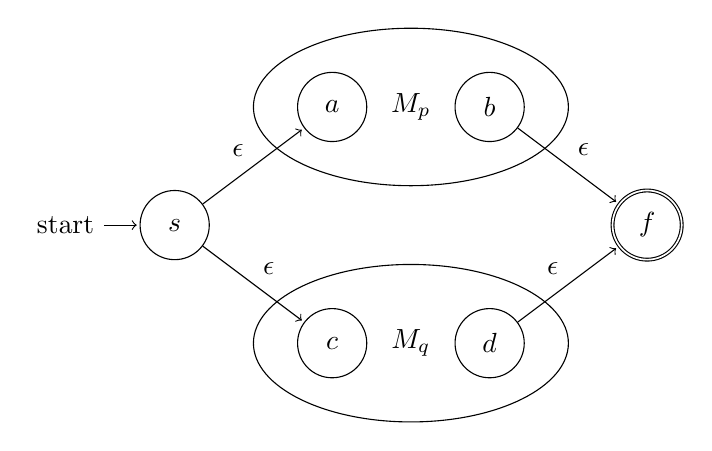
\begin{tikzpicture}[shorten >=1pt, auto]
      %\draw[help lines] (0,-3) grid (6,3);
      \draw (3,1.5) ellipse (2cm and 1cm) node {$M_p$};
      \draw (3,-1.5) ellipse (2cm and 1cm) node {$M_q$};
  
      \node[state, initial]   (s)             {$s$};
      \node[state]            (a) at (2,1.5)  {$a$};
      \node[state]            (b) at (4,1.5)  {$b$};
      \node[state]            (c) at (2,-1.5) {$c$};
      \node[state]            (d) at (4,-1.5) {$d$};
      \node[state, accepting] (f) at (6,0)    {$f$};
  
      \path[->] (s) edge node {$\epsilon$} (a)
                    edge node {$\epsilon$} (c)
                (b) edge node {$\epsilon$} (f)
                (d) edge node {$\epsilon$} (f);
    \end{tikzpicture}
    \caption{$M_{p+q}$}
  \end{figure}
  
  In $M_{p+q}$, the paths from a start state to an accepting state must contain
  a path from a start state in $M_p$ ($a$) to an accepting state in $M_p$ ($b$)
  or a path from a start state in $M_q$ ($c$) to an accepting state in $M_q$ 
  ($d$). Let $y_p$ be the set of labels of paths from some 
  
  So, the label, $y$, of such a path in $M_{p+q}$ is a 
   
  
  \item $p;q$:
  \begin{figure}[H]
    \centering
    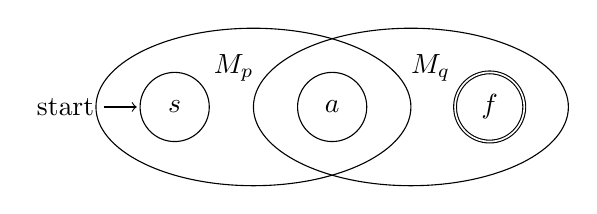
\begin{tikzpicture}[shorten >=1pt, auto]
      %\draw[help lines] (0,-3) grid (6,3);
      \draw (1,0) ellipse (2cm and 1cm);
      \draw (.75,.5) node {$M_p$};
      \draw (3,0) ellipse (2cm and 1cm);
      \draw (3.25,.5) node {$M_q$};
  
      \node[state, initial]   (s)           {$s$};
      \node[state]            (a) at (2,0)  {$a$};
      \node[state, accepting] (f) at (4,0)  {$f$};
    \end{tikzpicture}
    \caption{$M_{p;q}$}
  \end{figure}
  
  
  \item $p\star$:
  \begin{figure}[H]
    \centering
    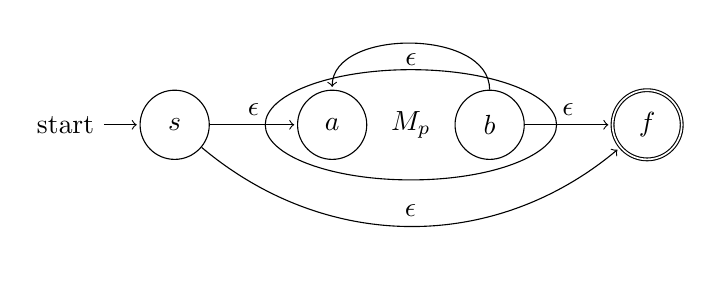
\begin{tikzpicture}[shorten >=1pt, auto]
      %\draw[help lines] (0,-3) grid (6,3);
      \draw (3,0) ellipse (1.85cm and .7cm) node {$M_p$};
  
      \node[state, initial]   (s)           {$s$};
      \node[state]            (a) at (2,0)  {$a$};
      \node[state]            (b) at (4,0)  {$b$};
      \node[state, accepting] (f) at (6,0)  {$f$};
  
      \path[->] (s) edge                 node {$\epsilon$} (a)
                    edge [bend right=40] node {$\epsilon$} (f)
                (b) edge [bend right=90] node {$\epsilon$} (a)
                    edge                 node {$\epsilon$} (f);
    \end{tikzpicture}
    \caption{$M_{p\star}$}
  \end{figure}
  
\end{itemize}
\end{description}
\end{proof}

\end{document}
